\documentclass[main.tex]{subfiles}
\section{Step size controller}

Ideally we would like to be able to obtain an accurate solution without having to take too many unnecesary steps. With this intention in mind we are going to modify the code, so that instead of having a fixed step size, we will give our method the ability to increase or decrease it depending on the error estimation.

Since we already know how to estimate the local error (step doubling or embbeded methods) we can check whether the error made for a specific step size is below a given tolerance. In case the error is larger than this tolerance, we reject the step and we update its size.

There are many ways one can control and update the step size. In our case we will make use of asymptotic and PI controllers. The former makes the update taking into account just the current value of the error, while the latter also relies on the previous estimation.

We have tested the five different methods for different values of the absolute and relative tolerances. The results using an asymptotic controller with relative and absolute tolerance of $10^{-3}$ are gathered in table \ref{tab:tol10e3}.


\begin{table}
\centering
\begin{tabular}{c|llll} \hline 
\multicolumn{5}{c}{Absolute tol $= 10^{-3}$ Relative tol $= 10^{-3}$} \\ \hline \hline
Method & Evaluations & Accepted & Rejected & \\ \hline 
Explicit Euler & 3175  & 1507 & 163 & \\ 
Implicit Euler & 21528 & 1490 & 186  & \\
Trapezoidal    & 18959 & 504  & 199 & \\
Runge-Kutta 4  & 10949  & 650  & 381 & \\
DROPI54        & 1749 & 178  & 85  & \\
\hline \hline 
\end{tabular}
\caption{Number of function evaluations number of steps accepted and number of steps rejected using an asymptotic controller}
\label{tab:tol10e3}
\end{table}

We see in table \ref{tab:tol10e3} that the number of function evaluations for the implicit methods is usually high. The reason is that this methods require a numerical solver, in this case Newton's method. It is also important to notice that, since DROPI54 uses an embedded method to estimate the error, the number of function evaluations is lower than for the rest of the methods, which compute those estimates by step doubling.


\begin{table}
\centering
\begin{tabular}{c|llll} \hline 
\multicolumn{5}{c}{Absolute tol $= 10^{-5}$ Relative tol $= 10^{-5}$} \\ \hline \hline
Method & Evaluations & Accepted & Rejected & \\ \hline 
Explicit Euler & 29847  & 14922 & 5   & \\ 
Implicit Euler & 139588 & 14860 & 5   & \\
Trapezoidal    & 47931  & 2190  & 133 & \\
Runge-Kutta 4  & 67155  & 6056  & 55  & \\
DROPI54        & 3487   & 380   & 139 & \\
\hline \hline 
\end{tabular}
\caption{Number of function evaluations number of steps accepted and number of steps rejected using an asymptotic controller}
\label{tab:tol10e5}
\end{table}

\begin{table}
\centering
\begin{tabular}{c|llll} \hline 
\multicolumn{5}{c}{Absolute tol $= 10^{-5}$ Relative tol $= 10^{-5}$} \\ \hline \hline
Method & Evaluations & Accepted & Rejected & \\ \hline 
Explicit Euler & 29856  & 14922 & 14    & \\ 
Implicit Euler & 139674 & 14860 & 15   & \\
Trapezoidal    & 54563  & 2202  & 443 & \\
Runge-Kutta 4  & 69431  & 6062  & 276 & \\
DROPI54        & 5734   & 383   & 510 & \\
\hline \hline 
\end{tabular}
\caption{Number of function evaluations number of steps accepted and number of steps rejected using a PI controller}
\label{tab:tol10e5PI}
\end{table}

We have also collected the results obtained for both asymptotic and PI controller with absolute and relative tolerances of $10^{-5}$ in tables \ref{tab:tol10e5} and \ref{tab:tol10e5PI}. The results show that there is not much difference between the two updating methods apart from the fact that PI takes a few more steps than the asymptotic controller. The top left graph reveals how for all the accepted points the residual coefficient is below 1 which corresponds to the tolerance especified, while all points above the treshold are rejected. 

\begin{table}
\centering
\begin{tabular}{c|llll} \hline 
\multicolumn{5}{c}{Absolute tol $= 10^{-8}$ Relative tol $= 10^{-8}$} \\ \hline \hline
Method & Evaluations & Accepted & Rejected & \\ \hline 
Explicit Euler & 943470  & 471728 & 17   & \\ 
Implicit Euler & 4621862 & 730992 & 65   & \\
Trapezoidal    & 350341  & 24438  & 367 & \\
Runge-Kutta 4  & 2118392 & 192553 & 32  & \\
DROPI54        & 13772    & 1389  & 676 & \\
\hline \hline 
\end{tabular}
\caption{Number of function evaluations number of steps accepted and number of steps rejected using a PI controller}
\label{tab:tol10e8}
\end{table} 

Table \ref{tab:tol10e8} shows the values obtained for absolute and relative tolerances of $10^{-8}$ with a PI controller. In this case the number of steps required for all methods except DOPRI54 is extremely large. That is why for such small tolerances high order methods are useful in order to prevent long run time and increase the computing performance.

\begin{figure}[H]
    \centering
    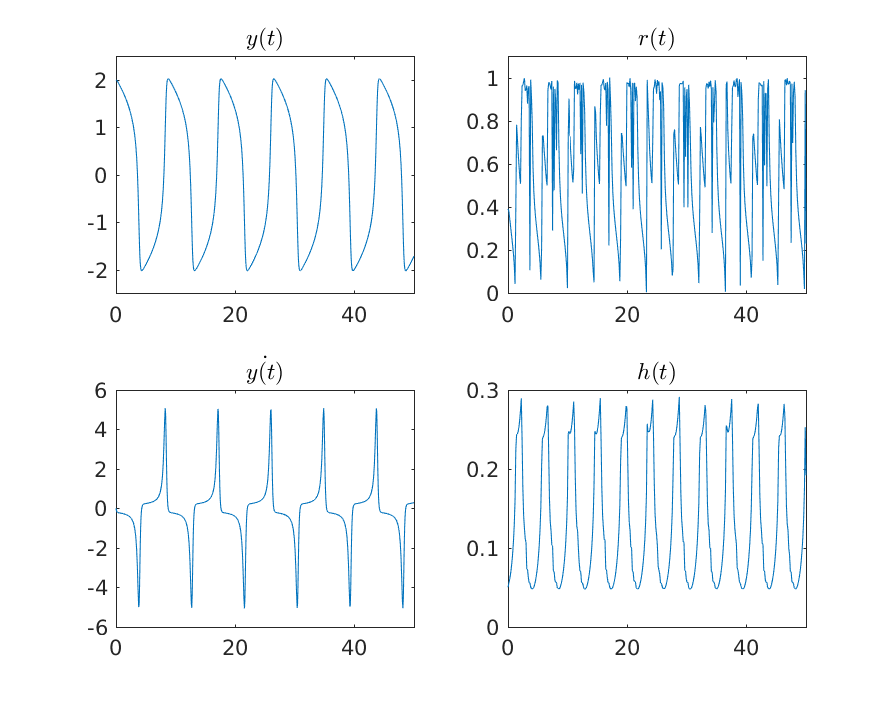
\includegraphics[width=\textwidth,clip]{../Figures/AdaptiveStepDOPRI54}
    \caption{Solution of the Van der Pol oscillator for DOPRI 54 with adaptive step size.}
    \label{fig:AdaptiveStep}
\end{figure}

Finally figure \ref{fig:AdaptiveStep} shows the solution found with DOPRI54, along with the step sizes chosen at every point in time. As expected, the closer the points are to the drops shown in the top left graph the more steps are needed to obtain an accurate solution and the shorter those steps are.